\chapter{Related Work}\label{ch:relatedwork}

We can now turn our attention to the current support for interfacing with the PMU in seL4, which prominently facilitates benchmarking in the kernel. Then, we will explore the performance subsystem on Linux, looking at both the user-space API, and how it is implemented.

\section{seL4 Benchmarking}

\subsection{Benchmarking}

The aim of benchmarking is twofold: (1) to detect performance regressions and (2) to identify opportunities for improvement. Benchmarking often takes the form as a suite of tests that are able to measure the performance of a given system. Benchmarking can be divided into standard and ad-hoc benchmarks. Standard benchmarks are designed by experts in the industry and tend to be based on macro-benchmarks, which attempt to represent real-world performance. The benefit of standardised benchmarks is that it provides a common standard, such that results can be compared. One example of a standardised benchmark is SPEC CPU 2017, which is designed to measure compute-intensive performance on a CPU \cite{SPECCPU2017}.

\subsection{sel4bench}

The repo sel4bench provides multiple applications for benchmarking different paths in the kernel \cite{GithubSel4bench}. Most notably it contains an application that benchmarks the Inter-process Communication (IPC) mechanism in seL4. The benchmarks are ad-hoc, since seL4 is an experimental system and therefore none of the standardised benchmarks are compatible\footnote{Most benchmarking suites designed for operating systems target UNIX/POSIX like systems.}.

\subsection{libsel4bench Overview}\label{sect:libsel4bench}

Interfacing with the PMU directly via platform dependent assembly instructions and MSRs (see Section \ref{sect:programming_pmu}), while illuminating, requires further layers of abstraction before it can be useful to developers on seL4. 

The seL4 benchmarks require access to the PMU counters, specifically to count the number of CPU cycles required to perform a particular operation. How CPU cycles, or any other PMU event is counted, depends on the underlying platform (e.g x86, ARM, RISC-V), as well as the specific architecture (e.g for ARM, this could be ARMv6, ARMv7, ARMv8 etc.) The libsel4bench library is designed to abstract over the performance monitoring counters (PMCs) \cite{github_libsel4bench_sel4bench_header}.

\subsection{libsel4bench Extensions}

In order for libsel4bench to also support benchmarking and profiling on seL4, support for additional PMU functionality will be required. 

\subsubsection{PMU Sampling Support}
Earlier, in Section \ref{sect:sampling_counting}, we saw that counting is when we are only interested in reading the PMU counters, compared to sampling where we configure the PMU to notify us when a counter has overflowed. While libsel4bench provides extensive support for counting, it does not provide any support for sampling the performance counters.

Sampling is not necessarily required for benchmarking in seL4, since often it is suffice to sample the counter value directly before and after the operation to be benchmarked. However, for a statistical profiler, sampling support is fundamental since it is the mechanism that switches control back to the profiler such that it can snapshot the running threads state (i.e PC, call stack, register set).

\section{Performance Counters for Linux (PCL)}\label{sect:pcl}

The PCL is a kernel-based subsystem that provides a framework for collecting and analysing performance data \cite{DocsRedHatPCL}. It is also commonly known in the open source community as Linux perf events (LPE), or \texttt{perf\_events} \cite{BlogBrendandGreggPerf}. The subsystem was merged into the Linux kernel in version 2.6.31 \cite{DocsUnofficialLinxPerfEvents} (most recent version is 5.17.4, released 20 April 2022). 

\subsection{The perf utility}

\begin{figure}[!h]
\centering
    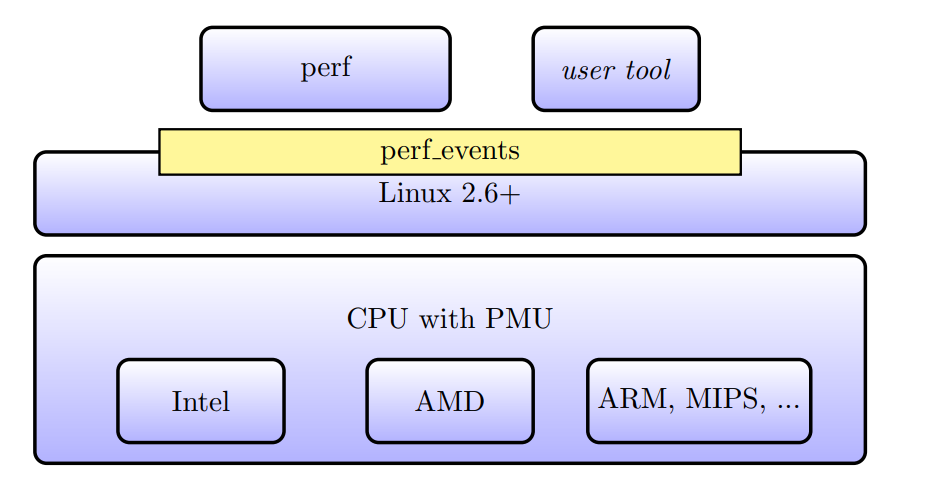
\includegraphics[width=0.8\linewidth]{report-a_perf_util_arch}
    \caption{How the perf utility relates to the PCL subsystem. Taken directly from Figure 1 in the CERN openlab, titled ``perf file format" \cite{CERN_openlab_perf_file_format}.}
    \label{fig:perf_util_arch}
\end{figure}

The perf utility is the Command Line Interface (CLI) to the PCL subsystem (\texttt{perf\_events}) \cite{ManPerfCLI}. It is a high level interface (see Figure \ref{fig:perf_util_arch}) that acts as an entry point for a number of commands, such as:

\ssp
\begin{itemize}
    \item \shellcmd{perf stat} - instruments and summarises key CPU counters (PMCs)
    \item \shellcmd{perf record} - records PMU events (to perf.data) which can be later reported
    \item \shellcmd{perf report} - breaks down events by process, function, etc. and allows user to filter events
    \item \shellcmd{perf annotate} - annotate assembly or source code with event counts
    \item \shellcmd{perf top} - view live event count (in realtime)
    \item \shellcmd{perf bench} - run benchmarks for different kernel subsystems
\end{itemize}
\dsp

\subsection{perf record}

The \shellcmd{perf record} command invokes the statistical profiler (see Section \ref{sect:statistical_profiling} for an overview of statistical profiling). 

\subsubsection{Example Usage}

To familiarise ourself with the perf API, we will sample the CPU every 10000 instructions, such that we include the call stack in the sample, and filter out samples that were taken while the CPU was executing in kernel mode. We can specify with the shell command \shellcmd{perf record -g -e cycles:u -c 10000} where the argument:
\ssp
\begin{itemize}
    \item \texttt{-g} specifies that call stack should be included,
    \item \texttt{-e} specifies the sampling event,
    \item \texttt{-c} specifies the count at which a sample occurs. 
\end{itemize}
\dsp

However, when CPU cycles is the sampling event, it is often more convenient to sample based on a sampling frequency (in Hz), \shellcmd{perf record -g -F 99 -all-user}, where the argument \texttt{-F} specifies the frequency to sample and \texttt{-all-user} specifies that to sample whilst CPU is in user-mode. 

\subsection{perf report}\label{sect:perf_report}

The perf report command is responsible displaying the profile data generated by perf record. Note, the term \textit{profile} refers to the data generated by the profiler. In the case of a statistical profiler, a profile is a sequence of samples.

\subsubsection{Example Report}

To help illustrate how perf report presents the profile data, we will profile a small C program that has a sufficiently complex call stack to demonstrate the nature of sampling. We can run perf record with the same arguments as before, but we also pass the program to profile with \shellcmd{perf record -g -e cycles:u -c 10000 simple\_prog}.

\subsubsection{Interpreting the Report}

Once the program has finished executing, we can run \shellcmd{perf report}. This displays the output depicted in Figure \ref{fig:perf_report_output}:

\begin{figure}[!h]
    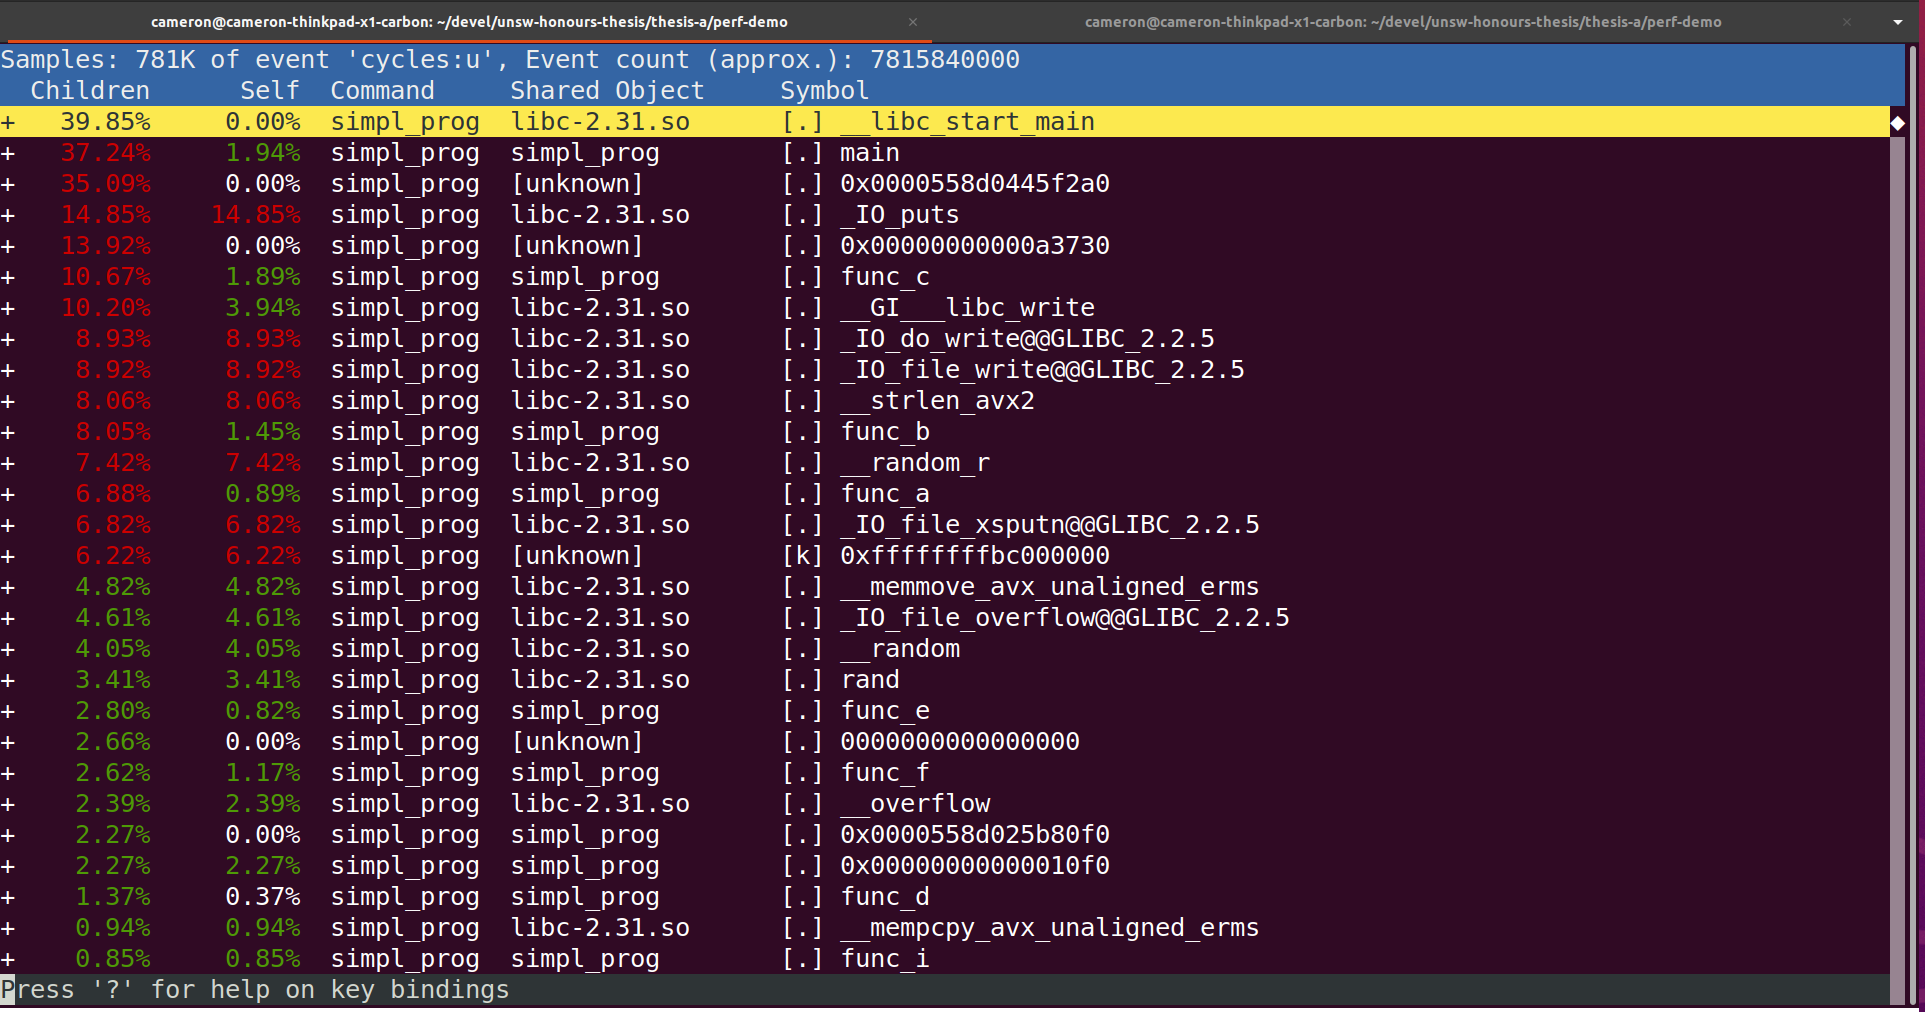
\includegraphics[width=\linewidth]{thesis-a_perf_report}
    \caption{Example output from \shellcmd{perf report}.}
    \label{fig:perf_report_output}
\end{figure}

By default, the table in the report is separated into five columns:

\ssp
\begin{itemize}
    \item \textit{Children} is the percentage of overall samples that were collected exclusively within a descendant function.
    \item \textit{Self} is the percentage of overall samples that were collected within the function itself (i.e ignoring descendant functions).
    \item \textit{Command} is the process the samples were collected from.
    \item \textit{Shared Object} displays the name of the Executable and Linkable Format (ELF) image where the samples came from.
    \item \textit{Symbol} displays the name of the function that was executing when the sample was taken.
\end{itemize}
\dsp

In the example report, there are a number of notable points:
\ssp
\begin{enumerate}
    \item The ``Children" and ``Self" columns are percentage values, and do not represent time, but rather percentage of overall samples. If the total execution time for the profile is known, the cumulative execution time for a given function can be approximated using the number of samples where the function appears. 
    \item The ``Shared Object" column refers to ELF images other than simple\_prog. This is because there are calls to libc functions, namely \texttt{time}, \texttt{srand}, \texttt{getpid} and \texttt{printf} which are still executing within the simple\_prog process address space.
    \item Instances where the value for ``Shared Object'' show \texttt{[unknown]} refer to dynamic shared objects (DSO), where the object name could not be resolved.
    \item The cases where the value for ``Shared Object'' is simple\_prog, but the corresponding symbol is a raw address, is due to the profiler not being able to find an entry in the ELF image for that particular address.
    \item Lastly, if we were to count all (CPU) cycles, instead of only user cycles, we would expect to see kernel symbols also appearing in the report.
\end{enumerate}
\dsp

\subsection{Event Groupings}\label{sect:event_groupings}

The PCL subsystem allows events to be grouped. A group of events are atomically assigned to PMU counters, in that at any given point in time, either they are all actively being counted by the PMU, or none are. This ensures that each event in the group was active for the identical number of CPU instructions, which is required in order to correctly compute ratios being two events. For example, number of L1 cache misses per instruction software increment.

\subsection{PCL User-level Interface}\label{sect:perf_event_open}

On Linux, the \texttt{perf} utility somehow needs to interact with the PCL subsystem, which it does so via the \texttt{perf\_events\_open} syscall in Listing \ref{lst:perf_events_open_syscall}.

\begin{listing}
    \begin{minted}{C}
int syscall(SYS_perf_event_open, struct perf_event_attr *attr,
            pid_t pid, int cpu, int group_fd, unsigned long flags);
    \end{minted}
    \caption{User-level syscall to interface with PCL subsystem}
    \label{lst:perf_events_open_syscall}
\end{listing}

The arguments for the syscall are:
\ssp\begin{itemize}
    \item \texttt{SYS\_perf\_event\_open} is an integer defined in \texttt{<sys/syscall.h>} that uniquely identifies the syscall within the kernel.
    \item \texttt{struct perf\_event\_attr *attr} is a pointer to the \texttt{struct} that provides detailed configuration information for the event to be measured. 
    \item \texttt{pid} is the process ID to measure.
    \item \texttt{cpu} is the CPU to measure.
    \item \texttt{group\_fd} allows event groups to be created (see Section \ref{sect:event_groupings}).
    \item \texttt{flags} is formed by ORing a number of flags that prominently alter how the returned file descriptor should behave.
\end{itemize}\dsp

On success, the syscall returns a file descriptor (fd), which directly corresponds to a single event being measured. Events can then be enabled or disabled via the \texttt{ioctrl} or \texttt{prctrl} system calls. The PCL subsystem supports both counting and sampling events from user-space (see Section \ref{sect:sampling_counting} for an overview on the difference). 

\subsubsection{Counting Events}

Once the file descriptor (\texttt{fd}) for an event has been opened, the current value can obtained by reading from the \texttt{fd}. This typically is achieved via the \texttt{read} syscall, where the data read into the provided buffer (if the event is not grouped) will be an instance of \texttt{struct read\_format} (defined in Listing \ref{lst:struct_read_format}).

\begin{listing}
    \begin{minted}{C}
struct read_format {
    u64 value;         /* The value of the event */
    u64 time_enabled;  /* if PERF_FORMAT_TOTAL_TIME_ENABLED */
    u64 time_running;  /* if PERF_FORMAT_TOTAL_TIME_RUNNING */
    u64 id;            /* if PERF_FORMAT_ID */
};
    \end{minted}
    \caption{Data returned from reading the \texttt{fd} for an event.}
    \label{lst:struct_read_format}
\end{listing}

\subsubsection{Sampling Events}

Sampling an event differs from counting an event, in that the kernel will notify userspace every N events, where N is determined by the sampling frequency. The mechanism for notifying is via either a signal sent to the user process or by polling the file descriptor (e.g using \texttt{epoll}). Instead of reading directly from the file descriptor, the kernel will write records to a shared ring-buffer, which can then be accessed in user-space via \texttt{mmap}. A record, which is perhaps confusingly referred to as an asynchronous event in the man pages, can be one of 21 types. Four common record types are defined below:

\ssp
\begin{itemize}
    \item \texttt{PERF\_RECORD\_MMAP} indicates the \texttt{PROT\_EXEC} mappings. 
    \item \texttt{PERF\_RECORD\_COMM} indicates a change in the process name.
    \item \texttt{PERF\_RECORD\_LOST\_SAMPLES} indicates some number of samples may have been lost.
    \item \texttt{PERF\_RECORD\_SAMPLE} indicates a sample, which may contain the program counter, call stack, cpu, recent branch stack, register set etc. 
\end{itemize}
\dsp

\subsection{The perf File Format}\label{sect:perf_file_format}

The \shellcmd{perf record} command, by default, will write the profile data out to file called \texttt{perf.data}, which is then consumed by other perf tools (e.g \shellcmd{perf report}). In order to ensure interoperability, there is a perf file format which specifies the layout of data within the \texttt{perf.data} file, and is designed in such a way that it provides forwards and backwards compatibility \cite{GithubPerfFileFormat}.

The CERN openlab technical report from 2011 \cite{CERN_openlab_perf_file_format} covers the perf file format in depth. The format, as of April 2022, still largely resembles the format described in the report and therefore provides an excellent reference point, complimenting the documentation within the Linux repo itself \cite{GithubPerfFileFormat}.

The file format begins with a header, and defines an offset into the file for sections that store the event types that make up the profile, the attributes for each sampled event, and the recorded samples for each event. The file format essentially defines a way to serialise the event configuration from each \texttt{perf\_event\_open} syscall, as well as each sample that is placed into the shared buffer (see Figure \ref{fig:perf_design}). 

\begin{figure}[!h]
\centering
    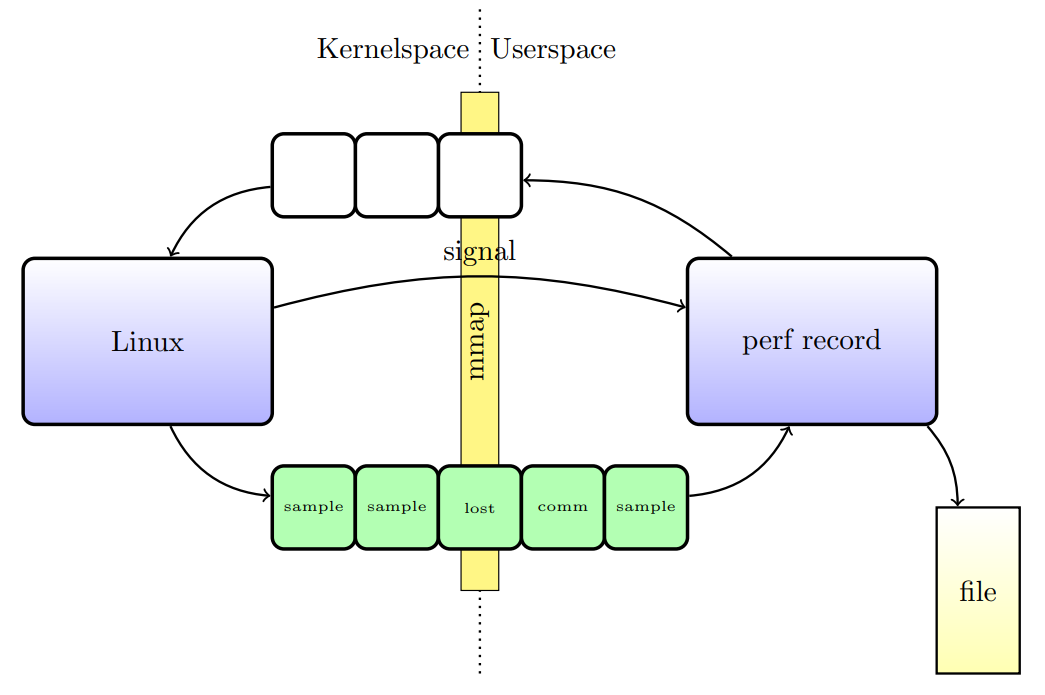
\includegraphics[width=0.8\linewidth]{report-a_perf_design}
    \caption{Overview of how the PCL subsystem (labelled as Linux) and the perf utility interact. Taken directly from Figure 2 in the CERN openlab, titled ``perf file format" \cite{CERN_openlab_perf_file_format}.}
    \label{fig:perf_design}
\end{figure}

